\documentclass[a4paper,11pt]{article}

\usepackage{pmisubmit}
\usepackage{graphicx}
\usepackage{breqn}
\begin{document}

\initpmisubmision{1} % assignment number
{Shashank Shailabh}   % your name
{170655}	% your roll number

\begin{pmisolution}
Given \hspace{2em} \(p(x|\eta) = \mathcal{N}(x|0,\eta)\) \hspace{2em} and \hspace{2em} \(p(\eta|\gamma) = Exp(\eta|\gamma^{2}/2 )\), where \(\eta \in [0,\infty)\)
\\
\[p(x|\gamma) = \int_{0}^{\infty} p(x|\eta)p(\eta|\gamma)d\eta = \int_{0}^{\infty} \mathcal{N}(x|0,\eta)Exp(\eta|\gamma^{2}/2 )d\eta\]\\
 Calculate MGF of \(p(x|\gamma)\)\\
 \begin{align*}
     M_{X}(t) &= \int_{-\infty}^{\infty} e^{tx}p(x|\gamma)dx\\
     &= \int_{-\infty}^{\infty}e^{tx} \int_{0}^{\infty} \mathcal{N}(x|0,\eta)Exp(\eta|\gamma^{2}/2 )dx d\eta\\
    &= \int_{0}^{\infty}Exp(\eta|\gamma^{2}/2)\left[\int_{-\infty}^{\infty}e^{tx}\mathcal{N}(x|0,\eta) dx\right]d\eta\\
    & &\pushright{\text{(Using MGF of Gaussian)}}\\
    &= \int_{0}^{\infty}\frac{\gamma^{2}}{2}e^{\frac{-\gamma^{2}\eta}{2}}\left[e^{\frac{t^{2}\eta}{2}}\right]d\eta\\
    &= \frac{\gamma^{2}}{2} \int_{0}^{\infty} e^{\frac{\eta(-\gamma^{2} + t^{2})}{2}}d\eta\\
    &= \frac{\gamma^{2}}{2} \left|\frac{2e^{\frac{\eta(-\gamma^{2} + t^{2})}{2}}}{(-\gamma^{2} + t^{2})} \right|_{0}^{\infty}\\
    &=  \begin{cases}
    \frac{1}{1- \frac{t^{2}}{\gamma^2}} &  \text{if   }    |t| < \gamma\\
    \infty &  \text{if   }  |t| \geq \gamma
  \end{cases}
 \end{align*}
 The above MGF is same as that of Laplace distribution \( L(\mu,b)\) having \(\mu = 0\) and \(b = \frac{1}{\gamma}\).\\\\
$p(x|\gamma)$ is marginal likelihood when $p(x|\eta)$ is likelihood and $p(\eta|\gamma)$ is prior distribution. It is summation of infinite number of gaussian distributions with different variance given by the exponential distribution. The intuition and plot shows that the Laplace(marginal likelihood) will have sharp peak than Gaussian (likelihood).
% \begin{wrapfigure}{r}{0.25\textwidth} %this figure will be at the right
%     \centering
%     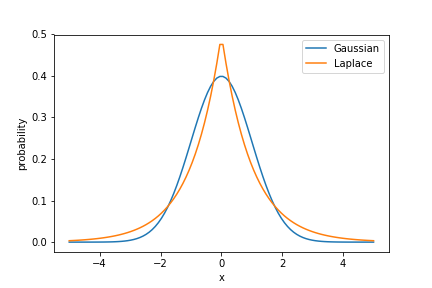
\includegraphics[width=0.25\textwidth]{question_1.png}
% \end{wrapfigure}
\begin{figure}[t]
\centering
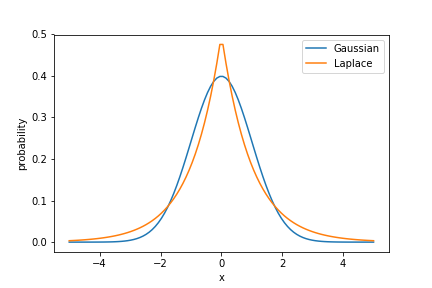
\includegraphics[height=2.2in]{question_1.png}
\caption{Probability distribution of Gaussian and Laplace.} 
%\info{refer this figure in the main text as well}}
\label{fig:q1}
\end{figure}
% \(M_{X}(t) = \int_{-\infty}^{\infty}e^{tx}p(x|\gamma)dx = \int_{-\infty}^{\infty}e^{tx} \int_{0}^{\infty} \mathcal{N}(x|0,\eta)Exp(\eta|\gamma^{2}/2 )d\eta\)\\
% \\
% \( M_{X}(t) = \int_{0}^{\infty}Exp(\eta|\gamma^{2}/2 )\left[\int_{-\infty}^{\infty}e^{tx}\mathcal{N}(x|0,\eta) dx\right]d\eta\)\\


%A vector symbol $\vb$, a symbol in blackboard font $\bR$, a symbol in calligraphic font $\cA$, \red{some} \green{colored} \blue{text}
\end{pmisolution}


\begin{pmisolution} 
Posterior predictive distribution \(p(y_{\ast}|\vx_{\ast}) = \mathcal{N}(\mu_{N}^{T}\vx_{\ast}, \beta^{-1} \: + \: + \vx_{\ast}^{T}\sum_{N}\vx_{\ast})\) and \(\beta > 0\).\\
\\
Var(\(y_{\ast}|\vx_{\ast}) = \beta^{-1} + \vx_{\ast}^{T}\sum_{N}\vx_{\ast}\) \hfill where \(\sum_{N} = (\beta\sum_{n=1}^{N}\vx_{n}\vx_{n}^{T} + \lambda\vI)^{-1}\)\\
\\
Comparing variance for N and N-1 values,
 \begin{align*}
     var(y_{\ast}|\vx_{\ast})_{N} &= \beta^{-1} + \vx_{\ast}^{T}(\beta\sum_{n=1}^{N}\vx_{n}\vx_{n}^{T} + \lambda\vI)^{-1}\vx_{\ast} \\
     &= \beta^{-1} + \vx_{\ast}^{T}( \beta\vx_{N}\vx_{N}^{T} + \beta\sum_{n=1}^{N-1}\vx_{n}\vx_{n}^{T} + \lambda\vI)^{-1}\vx_{\ast}\\
     & \text{(Using formula given in problem)}\\
     &= \beta^{-1}+\vx_{\ast}^{T}(\beta\sum_{n=1}^{N-1}\vx_{n}\vx_{n}^{T}+\lambda\vI)^{-1}\vx_{\ast} - \\
     & \left[ \frac{\vx_{\ast}^{T}\beta(\beta\sum_{n=1}^{N-1}\vx_{n}\vx_{n}^{T}+\lambda\vI)^{-1}\vx_{N}\vx_{N}^{T}(\beta\sum_{n=1}^{N-1}\vx_{n}\vx_{n}^{T}+\lambda\vI)^{-1}\vx_{\ast}}{1+\beta\vx_{N}^{T}(\beta\sum_{n=1}^{N-1}\vx_{n}\vx_{n}^{T}+\lambda\vI)^{-1}\vx_{N}}\right] \\
     &= var(y_{\ast}|\vx_{\ast})_{N-1} - \left[ \frac{\vx_{\ast}^{T}\beta(\beta\sum_{n=1}^{N-1}\vx_{n}\vx_{n}^{T} + \lambda\vI)^{-1}\vx_{N}\vx_{N}^{T}(\beta\sum_{n=1}^{N-1}\vx_{n}\vx_{n}^{T} + \lambda\vI)^{-1}\vx_{\ast}}{1 + \beta \vx_{N}^{T}(\beta\sum_{n=1}^{N-1}\vx_{n}\vx_{n}^{T} + \lambda\vI) ^{-1}\vx_{N}}\right]
 \end{align*}
 \begin{align*}
     var(y_{\ast}|\vx_{\ast})_{N} - var(y_{\ast}|\vx_{\ast})_{N-1} = - \left[ \frac{\vx_{\ast}^{T}\beta(\beta\sum_{n=1}^{N-1}\vx_{n}\vx_{n}^{T} + \lambda\vI)^{-1}\vx_{N}\vx_{N}^{T}(\beta\sum_{n=1}^{N-1}\vx_{n}\vx_{n}^{T} + \lambda\vI)^{-1}\vx_{\ast}}{1 + \beta \vx_{N}^{T}(\beta\sum_{n=1}^{N-1}\vx_{n}\vx_{n}^{T} + \lambda\vI) ^{-1}\vx_{N}}\right]\\
 \end{align*}
Now, finding whether the right side term will be postive or negative will gave our require result. Also, covariance matrix is symmetric and positive semi-definite matrix. \\
\\
The denominator looks is similar to \( 1+ \beta\vu^{T}\vS\vu\) where \(\vu\) is vector and \(\bS\) is the symmetric covariance PSD matrix. Using PSD property that \(\vu^{T}\vS\vu \geq 0\) \(\forall \: \vu\), hence the denominator is positive.\\
\\
Numerator can be written as a product of vector and its transpose:\\
\\
\(Numerator = -\beta [\vx_{\ast}^{T}(\beta\sum_{n=1}^{N-1}\vx_{n}\vx_{n}^{T} + \lambda\vI)^{-1}\vx_{N}][\vx_{\ast}^{T}(\beta\sum_{n=1}^{N-1}\vx_{n}\vx_{n}^{T} + \lambda\vI)^{-1}\vx_{N}]^{T}\)\\
\\
Using norm definition and property that norm is always non-negative for any vector:\\
\\
\(Numerator = -\beta ||\vx_{\ast}^{T}(\beta\sum_{n=1}^{N-1}\vx_{n}\vx_{n}^{T} + \lambda\vI)^{-1}\vx_{N}||^{2}\)\\
\\
Therefore, the numerator is multiplication of a negative and a non-negative value which results in non-positive for any value. \\
\\
It can also observed that covariance matrix of gaussian posterior is invertible and both \([x_{\ast},\vx_{N}\)vectors are non-zero so the norm vector will be non-zero. Using the norm property that zero vector has zero norm, it can be said that numerator will be negative and will not result in zero.
\\
\\
Since, \(\frac{numerator}{denominator}\) is negative so on increasing the number of training examples , the covariance of predictive posterior will decrease.

\end{pmisolution}

\begin{pmisolution}
$\vx = [x_{1} \: x_{2}\: .\: . \: . \: x_{N}]$ is the $N$ size vector of observations which are i.i.d from \(\mathcal{N}(x|\mu,\sigma^{2})\). \\
Consider a linear transformation on $\vx$ to obtain \(\bar{x} = \vS\vx + t\) where \(\bar{\vx} = \frac{1}{N}\sum_{x=1}^{N} x_{i}\), \(\vS =
\left[ {\begin{array}{c}
  \frac{1}{N} \\
  \frac{1}{N} \\
  . \\
  . \\
  . \\
  \frac{1}{N}\\
  \end{array} } \right]\)
%\left[\frac{1}{N} \: \frac{1}{N} \:. \:. \: \frac{1}{N}\right]\) 
is \(N \times 1\) size matrix and \(t=0\). \\
\\
Using gaussian properties for linear transformation on \(\bar{x}\)\\\\
Mean  = \(E[\bar{x}] = \vS E[\vx] + t\) \hfill where \(E[\bar{x}] = [\mu\: \mu\: .\:.\: . \: \mu\: ]\)\\
\\
\(E[\bar{x}] = \sum_{1}^{N} \frac{\mu}{N} = \mu \)\\
\\
Cov(\(\bar{x}\)) = \(\vS \sum \vS^{T}\) \hfill where \(\sum = \sigma^{2} I_{N}\) and \(I_{N}\) is identity matrix of size \(N\).\\
\\
Var(\(\bar{x}\)) = Cov(\(\bar{x}\)) = \(\frac{\sigma^{2}}{N}\)\\
Therefore, \(\bar{x}\) has a gaussian distribution with mean = \(\mu\) and variance = \(\frac{\sigma^{2}}{N}\). \\
\\
The intuition behind the above gaussian distribution is that increasing the number of training examples essentially decreases variance. Here, in the case of distribution of average of observations, we are averaging with the number of observations. Since the mean is same for all observation so new mean is also same. With increase in \(N\), we can provide more precise values.
\end{pmisolution}
%%%%%fourth question
\begin{pmisolution}
\section{First}
Likelihood given
\( p(\vx^{(m)}|\mu_{0},\sigma^{2}_{0}, \mu_{m}) = \prod_{n=1}^{N_{m}} \mathcal{N}(x_{n}^{(m)}| \mu_{m},\sigma^{2})\)\\
\\
Prior given
\( p(\mu_{m}|\mu_{0},\sigma^{2}_{0}) = \mathcal{N}(\mu_{m}| \mu_{0},\sigma^{2}_{0})\)\\

Since, prior and likelihood is gaussian and the their variance is constant. Using conjugacy, posterior will also be gaussian and calculation of marginal likelihood(intractable) is not needed. \\
\[p(\mu_{1},...,\mu_{M}|\vx,\mu_{0},\sigma^{2}_{0}) = \frac{p(\vx|\mu_{0},\sigma^{2}_{0}, \mu_{1},...,\mu_{M})p(\mu_{1},...,\mu_{M}|\mu_{0},\sigma^{2}_{0})}{p(\vx|\mu_{0},\sigma^{2}_{0},\sigma^{2})} \]
\[p(\mu_{1},...,\mu_{M}|\vx,\mu_{0},\sigma^{2}_{0}) \propto p(\vx|\mu_{0},\sigma^{2}_{0}, \mu_{1},...,\mu_{M})p(\mu_{1},...,\mu_{M}|\mu_{0},\sigma^{2}_{0}) \]
\[p(\mu_{1},...,\mu_{M}|\vx,\mu_{0},\sigma^{2}_{0}) \propto \left[ \prod_{n=1}^{N_{m}}\mathcal{N}(\vx_{n}^{(m)}| \mu_{m},\sigma^{2}) \right] \left[\prod_{m=1}^{M} \mathcal{N}(\mu_{m}| \mu_{0},\sigma^{2}_{0})\right] \]\\
\[p(\mu_{1},...,\mu_{M}|\vx,\mu_{0},\sigma^{2}_{0}) \propto \prod_{m=1}^{M} \left[ \prod_{n=1}^{N_{m}}\mathcal{N}(\vx_{n}^{(m)}| \mu_{m},\sigma^{2})\mathcal{N}(\mu_{m}| \mu_{0},\sigma^{2}_{0})\right]\]\\
Using squares trick, assume mean = \(\mu_{Am}\) and variance = \( \sigma_{Am}^{2}\)\\
Now, the value obtained for mean and variance \\
\[\mu_{Am} = \frac{\sigma^{2}\mu_{0}}{N_{m}\sigma_{0}^{2}+\sigma^{2}} + \frac{\sigma_{0}^{2}\sum_{n=1}^{N_{m}}x_{n}^{(m)}}{N_{m}\sigma_{0}^{2}+\sigma^{2}} \qquad \qquad \text{and} \qquad \qquad \frac{1}{\sigma_{Am}^{2}} = \frac{1}{\sigma_{0}^{2}} + \frac{N_{m}}{\sigma^{2}}\]
\[p(\mu_{1},...,\mu_{M}|\vx,\mu_{0},\sigma^{2}_{0}) = \prod_{m=1}^{M}\mathcal{N}(\mu_{m}|\mu_{Am}, \sigma_{Am}^{2}) \]
Therefore,
\[p(\mu_{m}|\vx,\mu_{0},\sigma^{2}_{0}) = \mathcal{N}(\mu_{m}|\mu_{Am}, \sigma_{Am}^{2}) \quad \forall \quad m =\{1,2,...,M\} \]
Thus, posterior mean is  \\
\( \mu_{Am} = \frac{\sigma^{2}\mu_{0}}{N_{m}\sigma_{0}^{2}+\sigma^{2}} + \frac{\sigma_{0}^{2}\sum_{n=1}^{N_{m}}x_{n}^{(m)}}{N_{m}\sigma_{0}^{2}+\sigma^{2}}\) and Variance is \( \sigma_{Am}^{2} = \left[ \frac{1}{\sigma_{0}^{2}} + \frac{N_{m}}{\sigma^{2}}\right]^{-1}\).
\section{Second}
Marginal likelihood can be calculated using prior, posterior and likelihood information.\\
\[ p(\vx|\mu_{0},\sigma^{2}_{0},\sigma^{2})= \frac{p(\vx|\mu_{0},\sigma^{2}_{0}, \mu_{1},...,\mu_{M})p(\mu_{1},...,\mu_{M}|\mu_{0},\sigma^{2}_{0})}{p(\mu_{1},...,\mu_{M}|\vx,\mu_{0},\sigma^{2}_{0})} \]
\[ p(\vx|\mu_{0},\sigma^{2}_{0},\sigma^{2}) =  \frac{\left[ \prod_{n=1}^{N_{m}}\mathcal{N}(\vx_{n}^{(m)}| \mu_{m},\sigma^{2}) \right] \left[\prod_{m=1}^{M} \mathcal{N}(\mu_{m}| \mu_{0},\sigma^{2}_{0})\right]}{\prod_{m=1}^{M}\mathcal{N}(\mu_{m}|\mu_{Am}, \sigma_{Am}^{2})} \]
Since our goal is \(\mu_{0}\) estimation, finding logarithm marginal likelihood and and removing all those terms which are independent of \(\mu_{0}\), \\
\[ \log p(\vx|\mu_{0},\sigma^{2}_{0},\sigma^{2}) = \sum_{m=1}^{M} \frac{1}{2}\left[ \frac{-1}{\sigma^{2}} \sum_{n=1}^{N_{m}}(x_{n}^{(m)}-\mu_{m})^{2} - \frac{1}{\sigma_{0}^{2}}(\mu_{m} - \mu_{0})^{2} + \frac{1}{\sigma_{Am}^{2}}(\mu_{m} - \mu_{Am})^{2}\right]\]
Differentiating the equation w.r.t. \(\mu_{0}\) yields,
\[ \hat{\mu} = \sum_{m=1}^{M} \frac{\sum_{n=1}^{N_{m}}x_{n}^{(m)}}{N_{m}} \]

Therefore, \(\hat{\mu} = \sum_{m=1}^{M} \frac{\sum_{n=1}^{N_{m}}x_{n}^{(m)}}{N_{m}}\) is the MLE-II estimate of \(\mu_{0}\).
\section{Third}
MLE-II is advantageous than using a known value because the former case use all the dataset and share information among schools simultaneously. A known value(due to human error) might be biased while MLE-II will not be biased.  
\end{pmisolution}

\begin{pmisolution}
Overall prior distribution can be obtained by product of prior of each school\\\\ \(p(\vw_{m}|\lambda) = \mathcal{N}(\vw_{m}| \vw_{0}, \lambda^{-1}\vI_{D}) \) and \(m = 1,2,...,M\)\\
\\
Similarly, likelihood can be obtained as\\
\\
\(p(\vy^{(m)}|\vX^{(m)},\vw_{m}, \beta) = \mathcal{N}(\vy^{(m)}|\vX^{(m)}\vw_{m}, \beta^{-1}\vI_{N}) \) and \(m = 1,2,...,M\) \\
\\
To calculate MLE-2 objective, calculate marginal likelihood expression using Gaussian Linear model property, \\
\(p(y|x) = \mathcal{N}(x,\vA\mu + b, \vA\mu+b,\vA\Lambda^{-1}\vA^{T}+\vL^{-1})\),
\\
\[p(\vy|\vX^{(1)},...,vX^{(M)},\vw_{1},...,\vw_{M}, \lambda,\vw_{0},\beta) = \prod_{m=1}^{M} \left[\int  \mathcal{N}(y_{m}|\vX^{(m)}\vw_{m}, \beta^{-1}\vI_{N}) \mathcal{N}(\vw_{m}| \vw_{0}| \lambda^{-1}, \vI_{D})\right]\]
\\
Now taking logarithm for MLE-2 calculation,\\
\[\log p(\vy|\vX^{(1)},...,\vX^{(M)},\vw_{1},...,\vw_{M}, \lambda,\vw_{0},\beta) = \sum_{m=1}^{M} \log \mathcal{N}(\vy^{(m)}|\vX^{(m)}\vw_{0},\lambda^{-1}\vX^{(m)}\vI_{D}\vX^{(m)T} + \beta^{-1}\vI_{N})\]

Therefore, \\
Objective = \(\sum_{m=1}^{M} \left[ \frac{-1}{2} (\vy^{(m)} - \vX^{(m)}\vw_{0})^{T}(\lambda^{-1}\vX^{(m)}\vX^{(m)T} + \beta^{-1}\vI_{N})^{-1}(\vy^{(m)} - \vX^{(m)}\vw_{0}) \right] + K\)\\
 where \(K\) is independent of \(\vw_{0}\). \\

One of the major benefit is that all the school's data is used in the calculation of \(w_{0}\) and it subsume all the dataset knowledge. Additionally, there is no need to carry validation for this and thus saving computation resources and time.
\end{pmisolution}
%%%%Sixth solution
\begin{pmisolution}
\textbf{Sol 1.} The below figures show the random functions drawn from the posterior for different values of K.  
\begin{figure}[h]
\centering
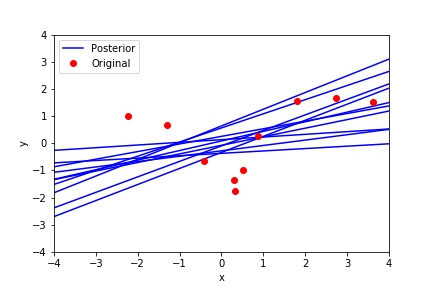
\includegraphics[height = 3.1in]{question_6a_1.png}
\caption{Posterior and original plots for K=1.} 
\end{figure}\begin{figure}[h]
\centering
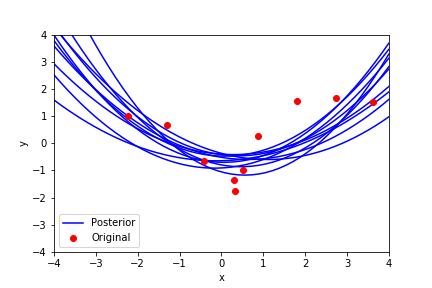
\includegraphics[height=3.1in]{question_6a_2.png}
\caption{Posterior and original plots for K=2.}
\end{figure}
\begin{figure}[h]
\centering
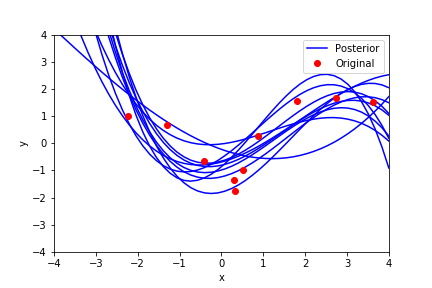
\includegraphics[height=3.1in]{question_6a_3.png}
\caption{Posterior and original plots for K=3.}
\end{figure}
\begin{figure}[h]
\centering
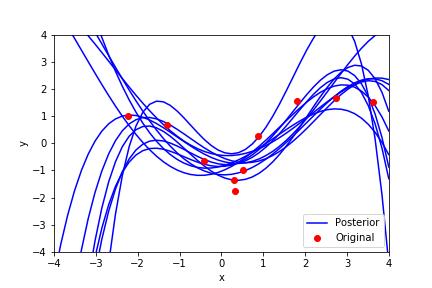
\includegraphics[height=3.1in]{question_6a_4.png}
\caption{Posterior and original plots for K=4.}
\end{figure}
\clearpage
\newpage
\textbf{Sol 2.} Below figures show the predictive mean and the grey region is the means plus minus twice of standard deviation.
\begin{figure}[h]
\centering
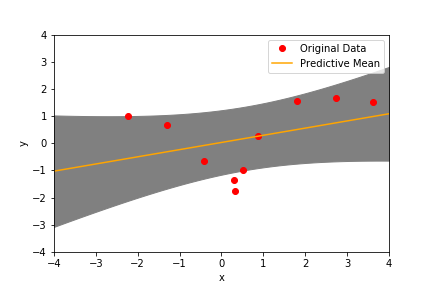
\includegraphics[height = 3.1in]{question_6b_1.png}
\caption{Predictive mean and original plots for K=1.} 
\end{figure}
\begin{figure}[h]
\centering
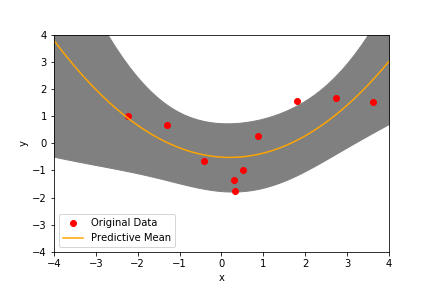
\includegraphics[height=3.1in]{question_6b_2.png}
\caption{Predictive mean and original plots for K=2.}
\end{figure}
\begin{figure}[h]
\centering
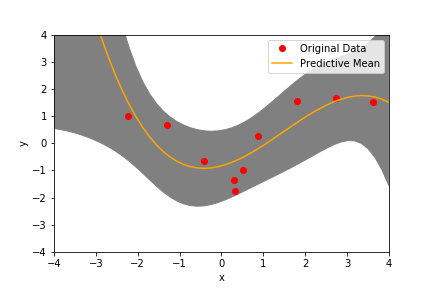
\includegraphics[height=3.1in]{question_6b_3.png}
\caption{Predictive and original plots for K=3.}
\end{figure}
\begin{figure}[h]
\centering
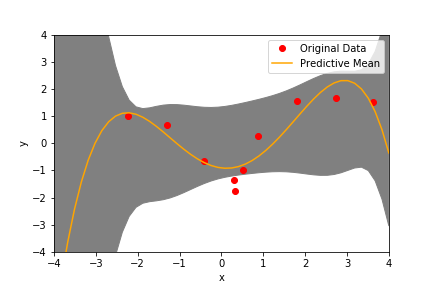
\includegraphics[height=3.1in]{question_6b_4.png}
\caption{ Predictive and original plots for K=4.}
\end{figure}
\clearpage
\newpage
\textbf{Sol 3.} The marginal log-likelihood for different values of K are -28.09, -15.35, 10.89 and -7.18 for K=1,2,3,4 respectively. K=4 explains the model best.\\
\\
\break
\textbf{Sol 4.} MAP estimate is mean of the posterior distribution. Log-likelihood for \(K = [1,2,3,4]\) values are \([-28.09,-15.36,-10.93,-7.23]\). K=4 attains the highest log-likelihood in all K values. Highest marginal log-likelihood is more reasonable since it captures the weights over all possible values while log-likelihood chooses one values (MAP estimate) hence, the former can be biased and not robust. Marginal-log likelihood also gives the uncertainty in the value. \\
\begin{figure}[h]
\centering
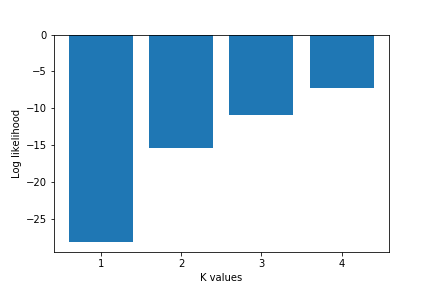
\includegraphics[height=3.1in]{question_6d.png}
\caption{ Log likelihood for different values of K.}
\end{figure}
\break
\textbf{Sol 5.} In predictive posterior, the models performs poor in x=[-4,-2.8] because of no training data. Hence, training data should be increased in this region to make better model. Increasing training data reduces the uncertainty in the model in that region.
\end{pmisolution}


\end{document}
